% !TEX root=../root.tex

In addition to the hardware results presented in the following section, we
present simulation results to show the effectiveness of the proposed estimation
algorithm.
A multirotor UAV is simulated using the dynamics presented
in~\eqref{eq:uav_dynamics}.
Additionally, a landing vehicle is simulated using the dynamics presented
in~\eqref{eq:goal_dynamics}. The standard deviations used for the zero-mean
Guassian noise processes in the dynamics are found
in~\tabref{tab:sim_process_noises}.
As the estimator depends on
tracking and estimating the positions of visual landmarks that are rigidly
attached to the landing vehicle, landmark positions on the landing vehicle
are also simulated.
Positions for each landmark in the goal frame are
randomly sampled from the
uniform distribution
\begin{equation}
  \vect{r}_{i/g}^g = \mathcal{U}
  \left( \begin{bmatrix} -2 \\ -2 \\ -1 \end{bmatrix},
  \begin{bmatrix} 2 \\ 2 \\ 1 \end{bmatrix} \right)
  \label{eq:uniform_dist}
\end{equation}
At each time step of the simulation, landmarks are given a one percent chance
of disappearing. When a landmark disappears, a new landmark is randomly
generated by sampling from~\eqref{eq:uniform_dist}.
A specified probability determines

The sensor measurements that are provided to the estimator are simulated using the true
state of the simulation. These sensor measurements include accelerometer,
gyroscope, global position of the UAV, global attitude 
of the UAV, relative position and attitude from the fiducial landing marker, and
landmark locations in the camera frame. All measurements are
corrupted with white Gaussian noise. The sensor noise parameters along with the
rate at which each sensor is sampled are found
in~\tabref{tab:sim_meas_noise}.

The landing vehicle was initialized with initial conditions of $v_x = 0.5
m/s$, $v_y = 0 m/s$, $\theta_I^g = 1.5 rad$ and $\omega = 0.5 rad/s$. The
simulated camera was oriented at a yaw angle of $\pi/2$ with respect to the body
frame and $p_{c/b}^b = \begin{bmatrix}0.25 & -0.2 &
0.4\end{bmatrix}^\transpose$.

The results for simulations where the estimator uses ten visual landmarks and
zero visual landmarks are seen in~\ref{fig:BLAH} and~\ref{fig:BLAH}
respectively. We do not include the plots of the UAV states,
$\vect{x}_{\text{UAV}}$, as it is well known that these states are easily
estimated with the given measurements. In the experiments shown in the plots,
the measurements from the fiducial landing marker are not used after $t = 5 s$
in the simulation to demonstrate the performance of the proposed estimation
algorithm. The figures clearly show that when ten visual landmarks are used by
the estimator, the estimates of the goal states remain accurate and consistent
throughout the duration of the simulation. However, when no visual landmarks are
used by the estimator, the estimate of the goal states quickly become incorrect.
We note that the $z$ direction of the goal position is the exception to this
because the landing vehicle is constrained to move only in the $xy$ plane.

To further demonstrate this performance, 100 simulation runs were performed
both using ten visual landmarks and using zero visual landmarks. The L2 norm of
the errors in the $x$ and $y$ direction of the goal position state are plotted
with respect to time in~\ref{fig:BLAH}. While the error when using ten landmarks
almost entirely remains under 1 m for all 100 simulations, the error when using
no landmarks quickly grows larger that 1 m. The error for several of the
simulations reaches over 10 m after 30s.

These simulation results clearly demonstrate the ability to maintain accurate
and consistent estimates of the goal states when the fiducial landing marker is
not detected for significant periods of time.


\begin{table}[h!]
  \begin{center}
    \caption{Simulation Motion Model Parameters.}
    \label{tab:sim_process_noises}
    \begin{tabular}{l|l}
      \textbf{Parameter} & \textbf{Std. Deviation} \\
      \hline
      $\vect{\eta}_{\beta_a}$ & 0.05 $m/s^2$ \\
      $\vect{\eta}_{\beta_\omega}$ & 0.01 $rad/s$ \\
      $\vect{\eta}_{gv}$ & 5 m/s \\
      $\vect{\eta}_{g\omega}$ & 5 rad/s \\
      % v & 5 m/s \\
      % landmark $x_{\text{min}}$ & -2 m \\
      % landmark $x_{\text{max}}$ & 2 m \\
      % landmark $y_{\text{min}}$ & -2 m \\
      % landmark $y_{\text{max}}$ & 2 m \\
      % landmark $z_{\text{min}}$ & -1 m \\
      % landmark $z_{\text{max}}$ & 1 m \\
      % landmark disappear prob. & 1\% \\
    \end{tabular}
  \end{center}
\end{table}

\begin{table}[h!]
  \begin{center}
    \caption{Simulation Sensor Noise Characteristics.}
    \label{tab:sim_meas_noise}
    \begin{tabular}{l|l|l}
      \textbf{Measurement} & \textbf{Std Dev} & \textbf{Rate} \\
      \hline
      Accelerometer & 0.2 $m/s^2$ & 250 Hz \\
      % walk & 0.05 $m/s^2$  \\
      % init & 0.01 $m/s^2$ \\
      Gyroscope & 0.1 $rad/s$ & 250 Hz \\
      % walk & 0.01 $rad/s$  \\
      % init & 0.01 $rad/s$ \\
      UAV global position & 0.01 $m$ & 10 Hz \\
      UAV global attitude & 0.001 $rad$ & 10 Hz \\
      Fiducial marker position & 0.1 $m$ & 30 Hz \\
      Fiducial marker attitude & 0.1 $rad$ & 30 Hz \\
      Landmark image point & 2.0 pixels & 30 Hz \\
    \end{tabular}
  \end{center}
\end{table}

\begin{figure}
  \centering
  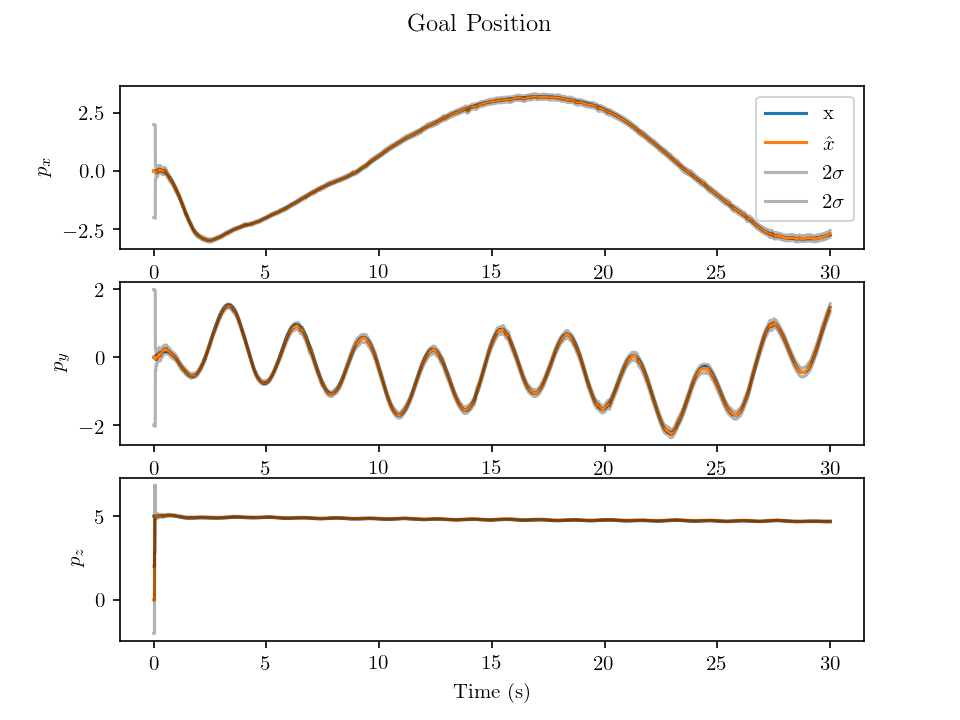
\includegraphics[scale=0.5]{plots/with_lms_gp.png}
  \caption{Simulation results with estimator using a maximum of ten visual
  landmarks. Measurements from the fiducial marker are not used after $t$ = 5
$s$ to demonstrate the performance of the estimator.}
  \label{fig:with_lms_gp}
\end{figure}

\begin{figure}
  \centering
  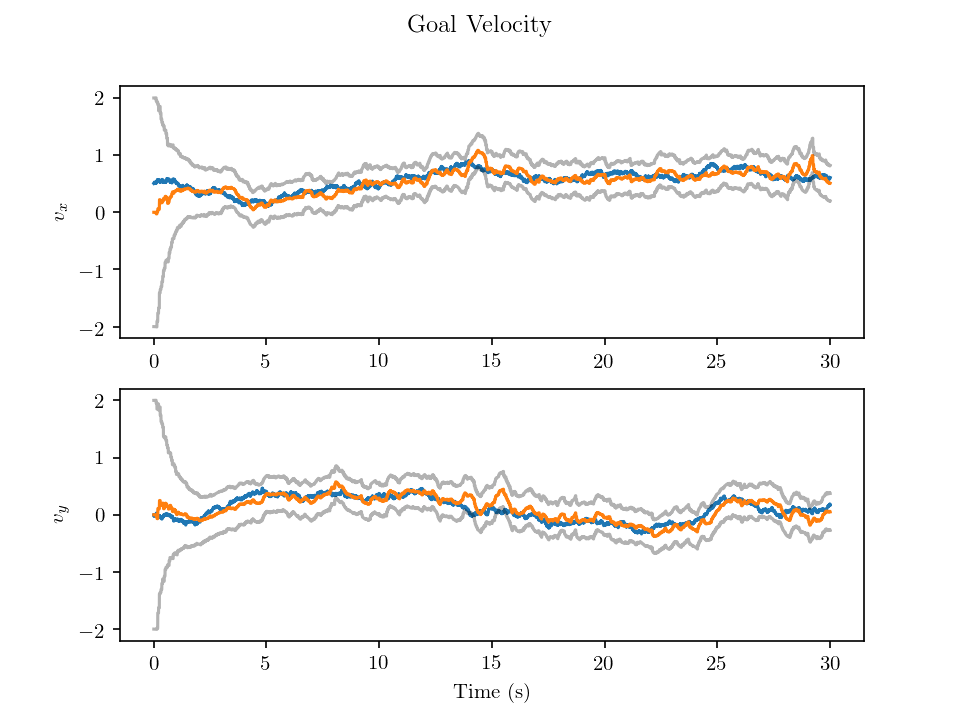
\includegraphics[scale=0.5]{plots/with_lms_gv.png}
  \caption{Simulation results with estimator using a maximum of ten visual
  landmarks. Measurements from the fiducial marker are not used after $t$ = 5
$s$ to demonstrate the performance of the estimator.}
  \label{fig:with_lms_gv}
\end{figure}

\begin{figure}
  \centering
  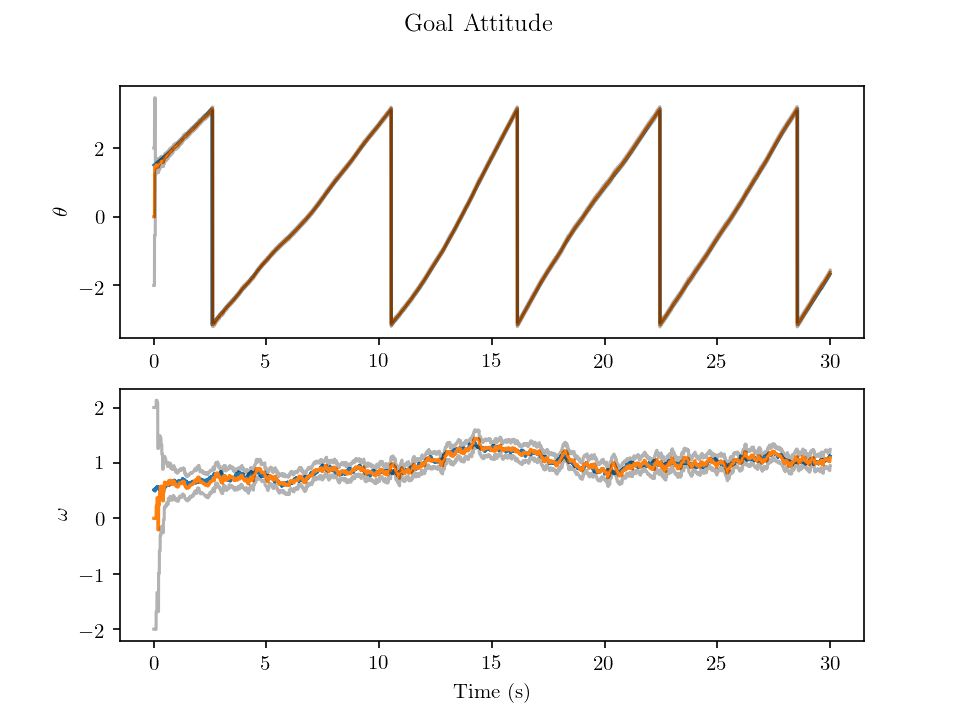
\includegraphics[scale=0.5]{plots/with_lms_gatt.png}
  \caption{Simulation results with estimator using a maximum of ten visual
  landmarks. Measurements from the fiducial marker are not used after $t$ = 5
$s$ to demonstrate the performance of the estimator.}
  \label{fig:with_lms_gatt}
\end{figure}

\begin{figure}
  \centering
  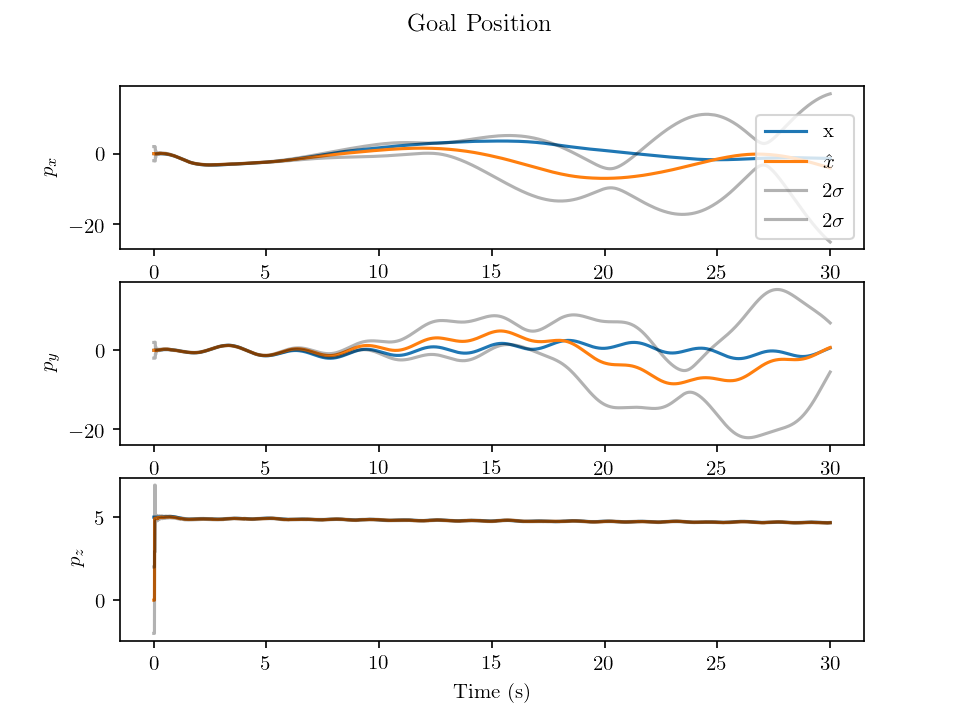
\includegraphics[scale=0.5]{plots/no_lms_gp.png}
  \caption{Simulation results with estimator using no visual
  landmarks. Measurements from the fiducial marker are not used after $t$ = 5
$s$ to demonstrate the performance of the estimator.}
  \label{fig:no_lms_gp}
\end{figure}

\begin{figure}
  \centering
  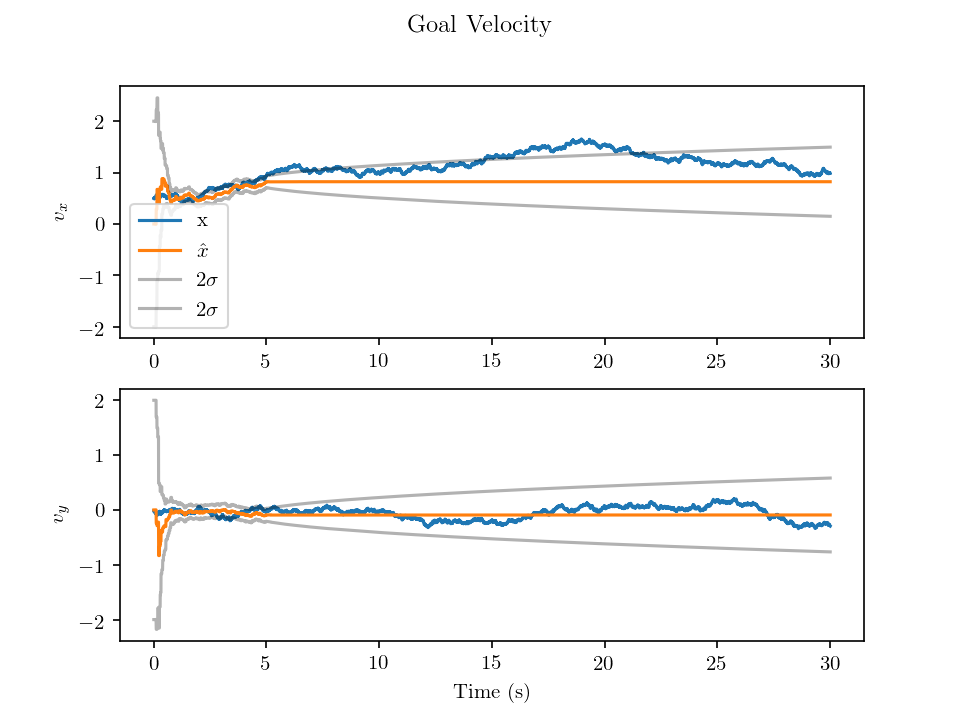
\includegraphics[scale=0.5]{plots/no_lms_gv.png}
  \caption{Simulation results with estimator using no visual
  landmarks. Measurements from the fiducial marker are not used after $t$ = 5
$s$ to demonstrate the performance of the estimator.}
  \label{fig:no_lms_gv}
\end{figure}

\begin{figure}
  \centering
  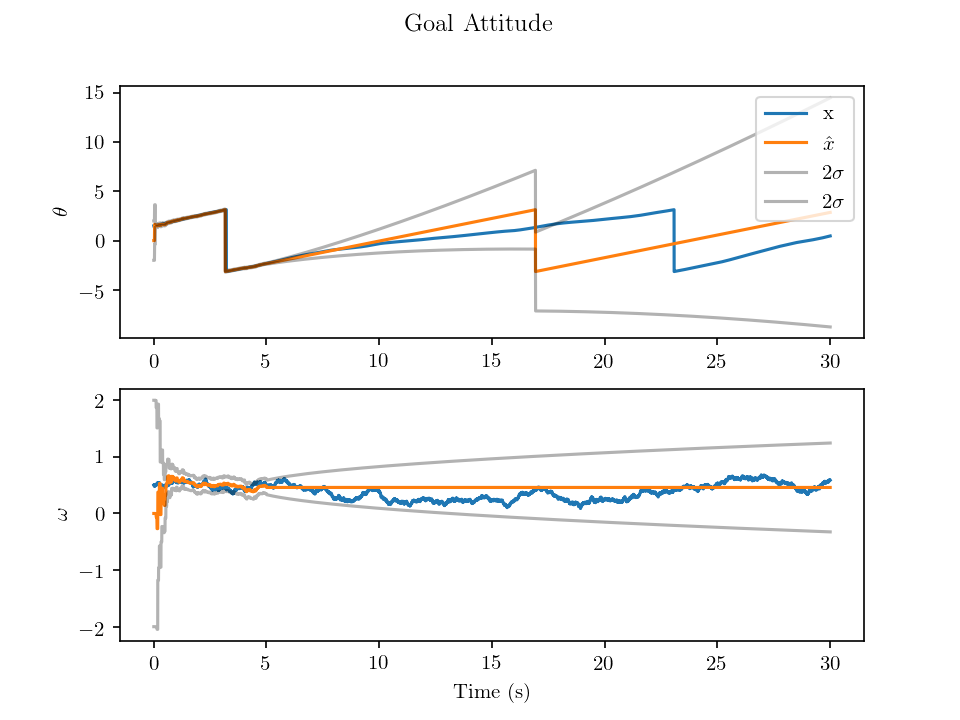
\includegraphics[scale=0.5]{plots/no_lms_gatt.png}
  \caption{Simulation results with estimator using no visual
  landmarks. Measurements from the fiducial marker are not used after $t$ = 5
$s$ to demonstrate the performance of the estimator.}
  \label{fig:no_lms_gatt}
\end{figure}

\begin{figure}
  \centering
  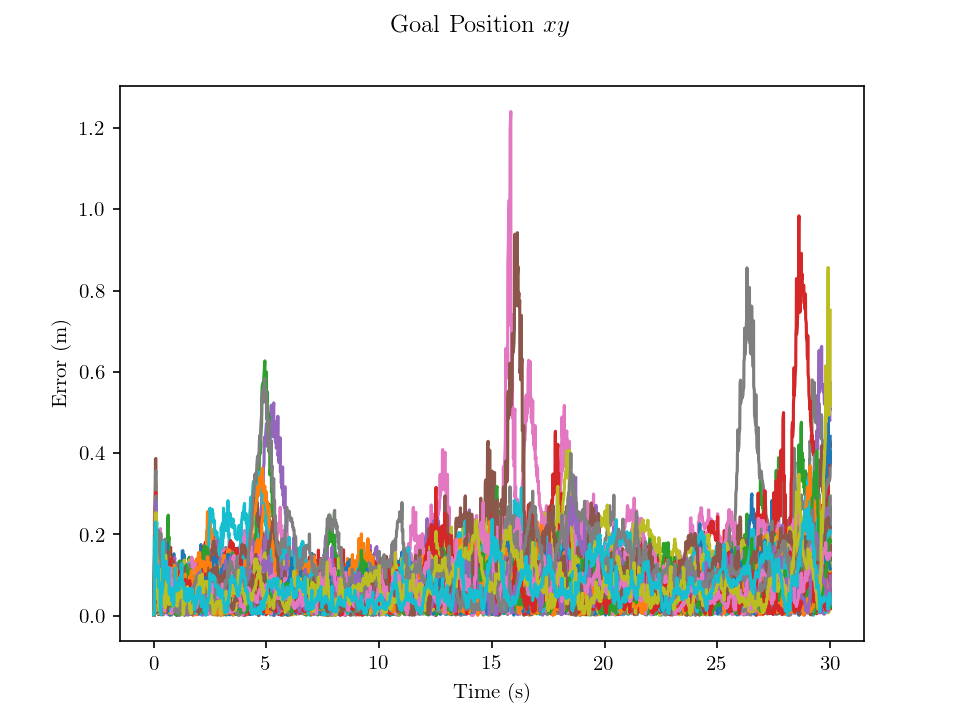
\includegraphics[scale=0.5]{plots/mc_with_lms_xy_err.png}
  \caption{Simulation results with estimator using a maximum of ten visual
  landmarks. Measurements from the fiducial marker are not used after $t$ = 5
$s$ to demonstrate the performance of the estimator. The L2 norm of the error in
the x and y directions of the goal position is seen for 100 different simulation
runs.}
  \label{fig:mc_with_lms_xy_err}
\end{figure}

\begin{figure}
  \centering
  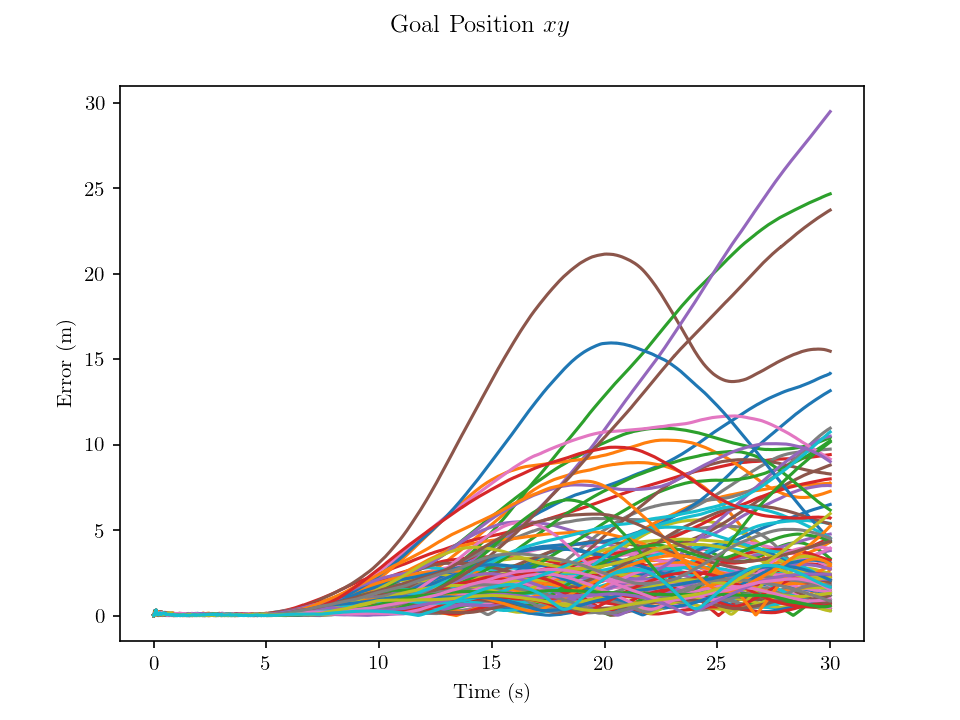
\includegraphics[scale=0.5]{plots/mc_no_lms_xy_err.png}
  \caption{Simulation results with estimator using no visual
  landmarks. Measurements from the fiducial marker are not used after $t$ = 5
$s$ to demonstrate the performance of the estimator. The L2 norm of the error in
the x and y directions of the goal position is seen for 100 different simulation
runs.}
  \label{fig:mc_no_lms_xy_err}
\end{figure}
